\documentclass[/home/jesse/Analysis/FemtoAnalysis/AnalysisNotes/AnalysisNoteJBuxton.tex]{subfiles}
\begin{document}

\subsubsection{\texorpdfstring{$\Lambda$K$^{+}$}{TEXT} Residuals}
\label{Residuals_LamKchP}

\begin{figure}[h]
  \centering
  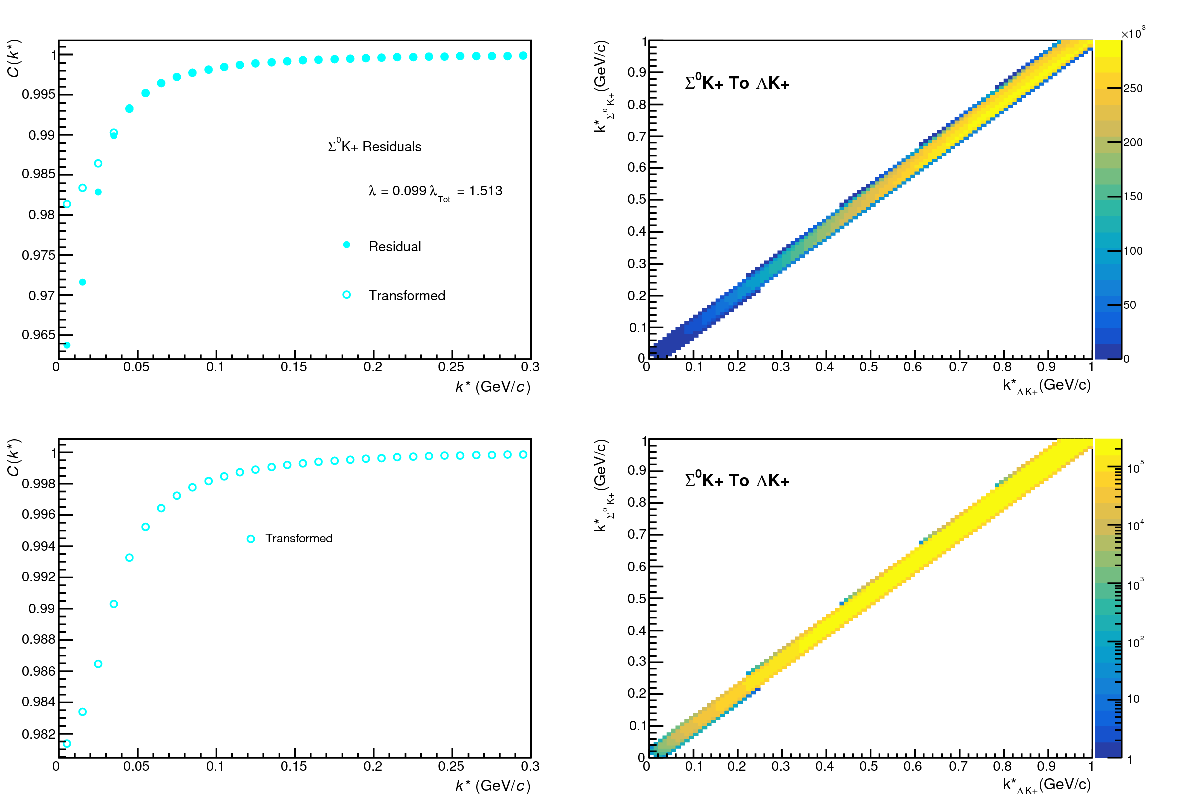
\includegraphics[width=\textwidth]{9_AdditionalFigures/Figures/Residuals/LamKchP/Residuals_LamKchP_0010_Sig0KchP_MomResCrctn_NonFlatBgdCrctn_10Res_PrimMaxDecay4fm_UsingXiDataAndCoulombOnly.pdf}
  \caption[Residuals: $\Sigma^{0}$K$^{+}$ to $\Lambda$K$^{+}$ (0-10\% Centrality)]{Residuals: $\Sigma^{0}$K$^{+}$ to $\Lambda$K$^{+}$ (0-10\% Centrality)}
  \label{fig:Res_LamKchP_0010_Sig0KchP}
\end{figure}


\begin{figure}[h]
  \centering
  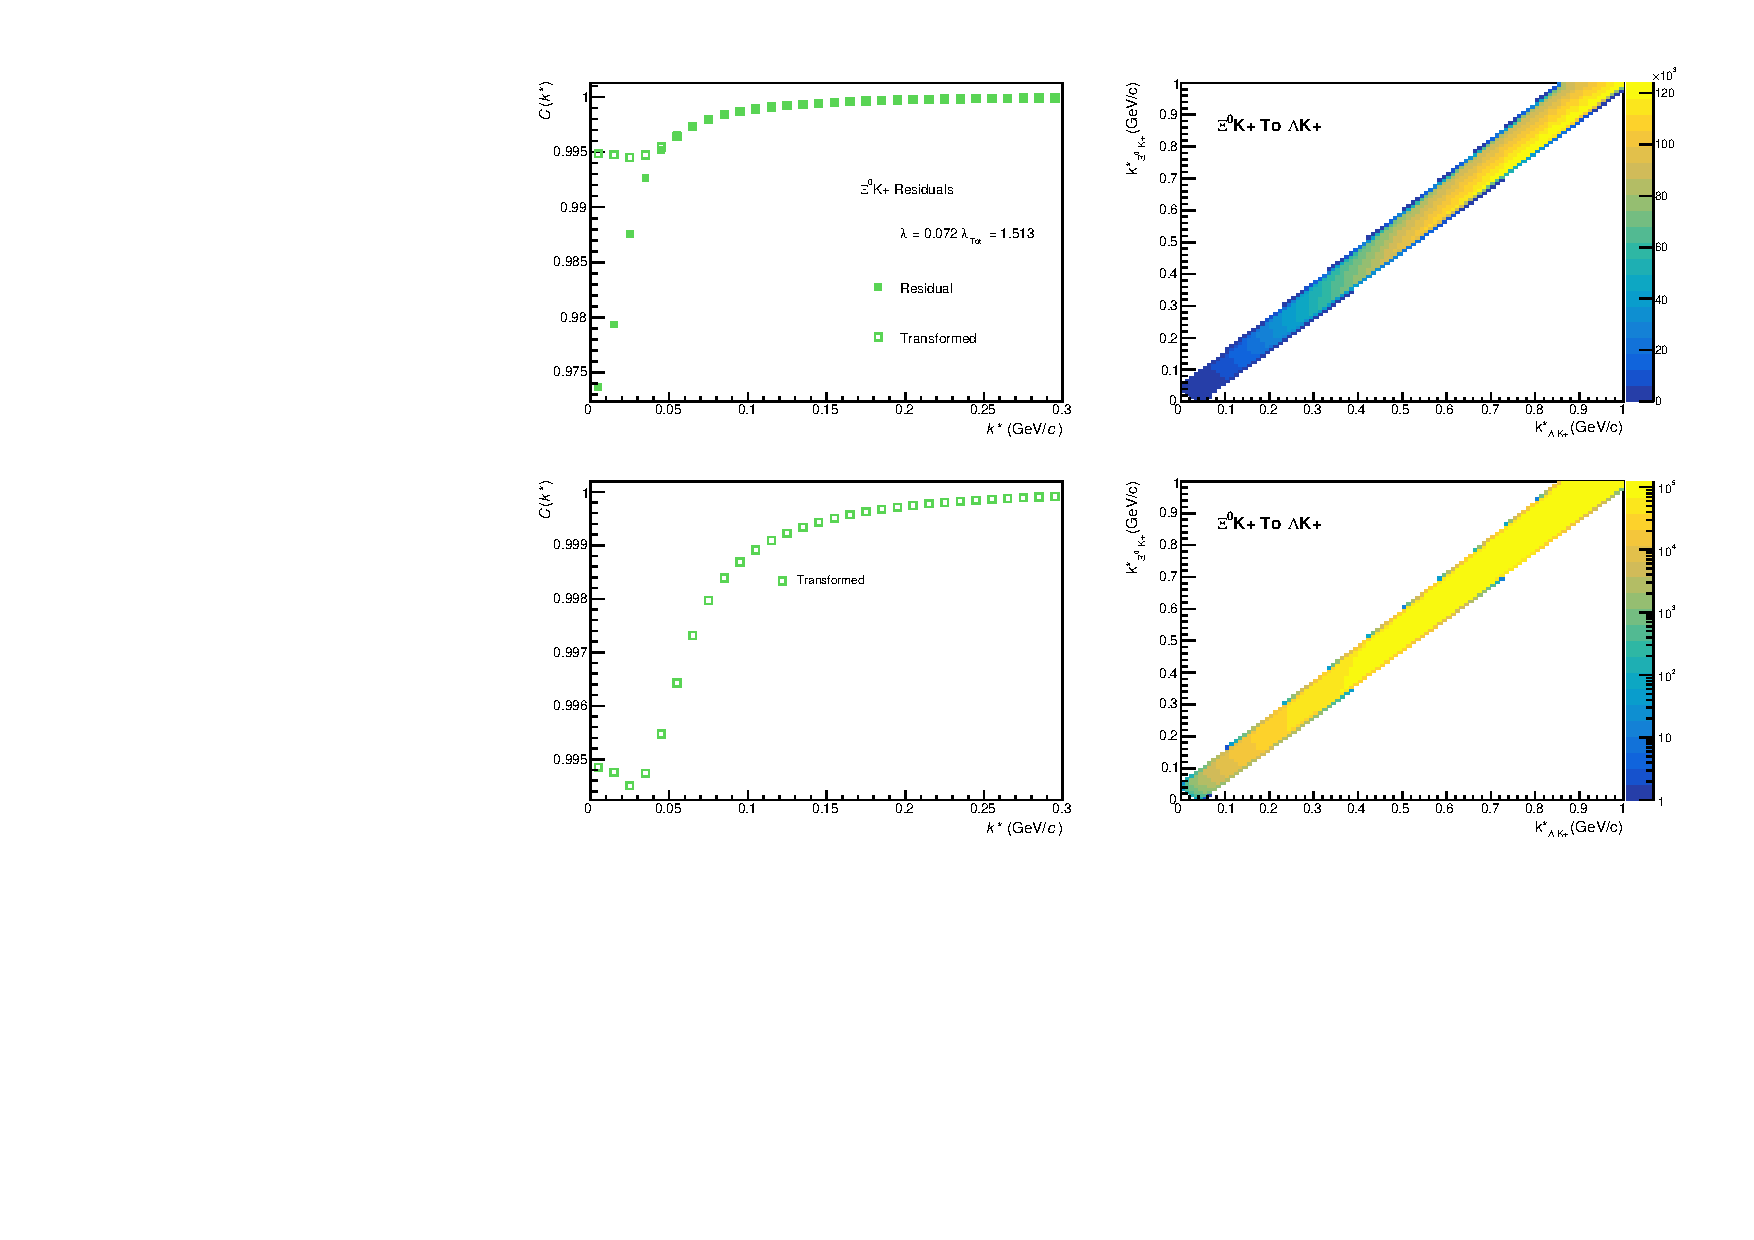
\includegraphics[width=\textwidth]{9_AdditionalFigures/Figures/Residuals/LamKchP/Residuals_LamKchP_0010_Xi0KchP_MomResCrctn_NonFlatBgdCrctn_10Res_PrimMaxDecay4fm_UsingXiDataAndCoulombOnly.pdf}
  \caption[Residuals: $\Xi^{0}$K$^{+}$ to $\Lambda$K$^{+}$ (0-10\% Centrality)]{Residuals: $\Xi^{0}$K$^{+}$ to $\Lambda$K$^{+}$ (0-10\% Centrality)}
  \label{fig:Res_LamKchP_0010_Xi0KchP}
\end{figure}


\begin{figure}[h]
  \centering
  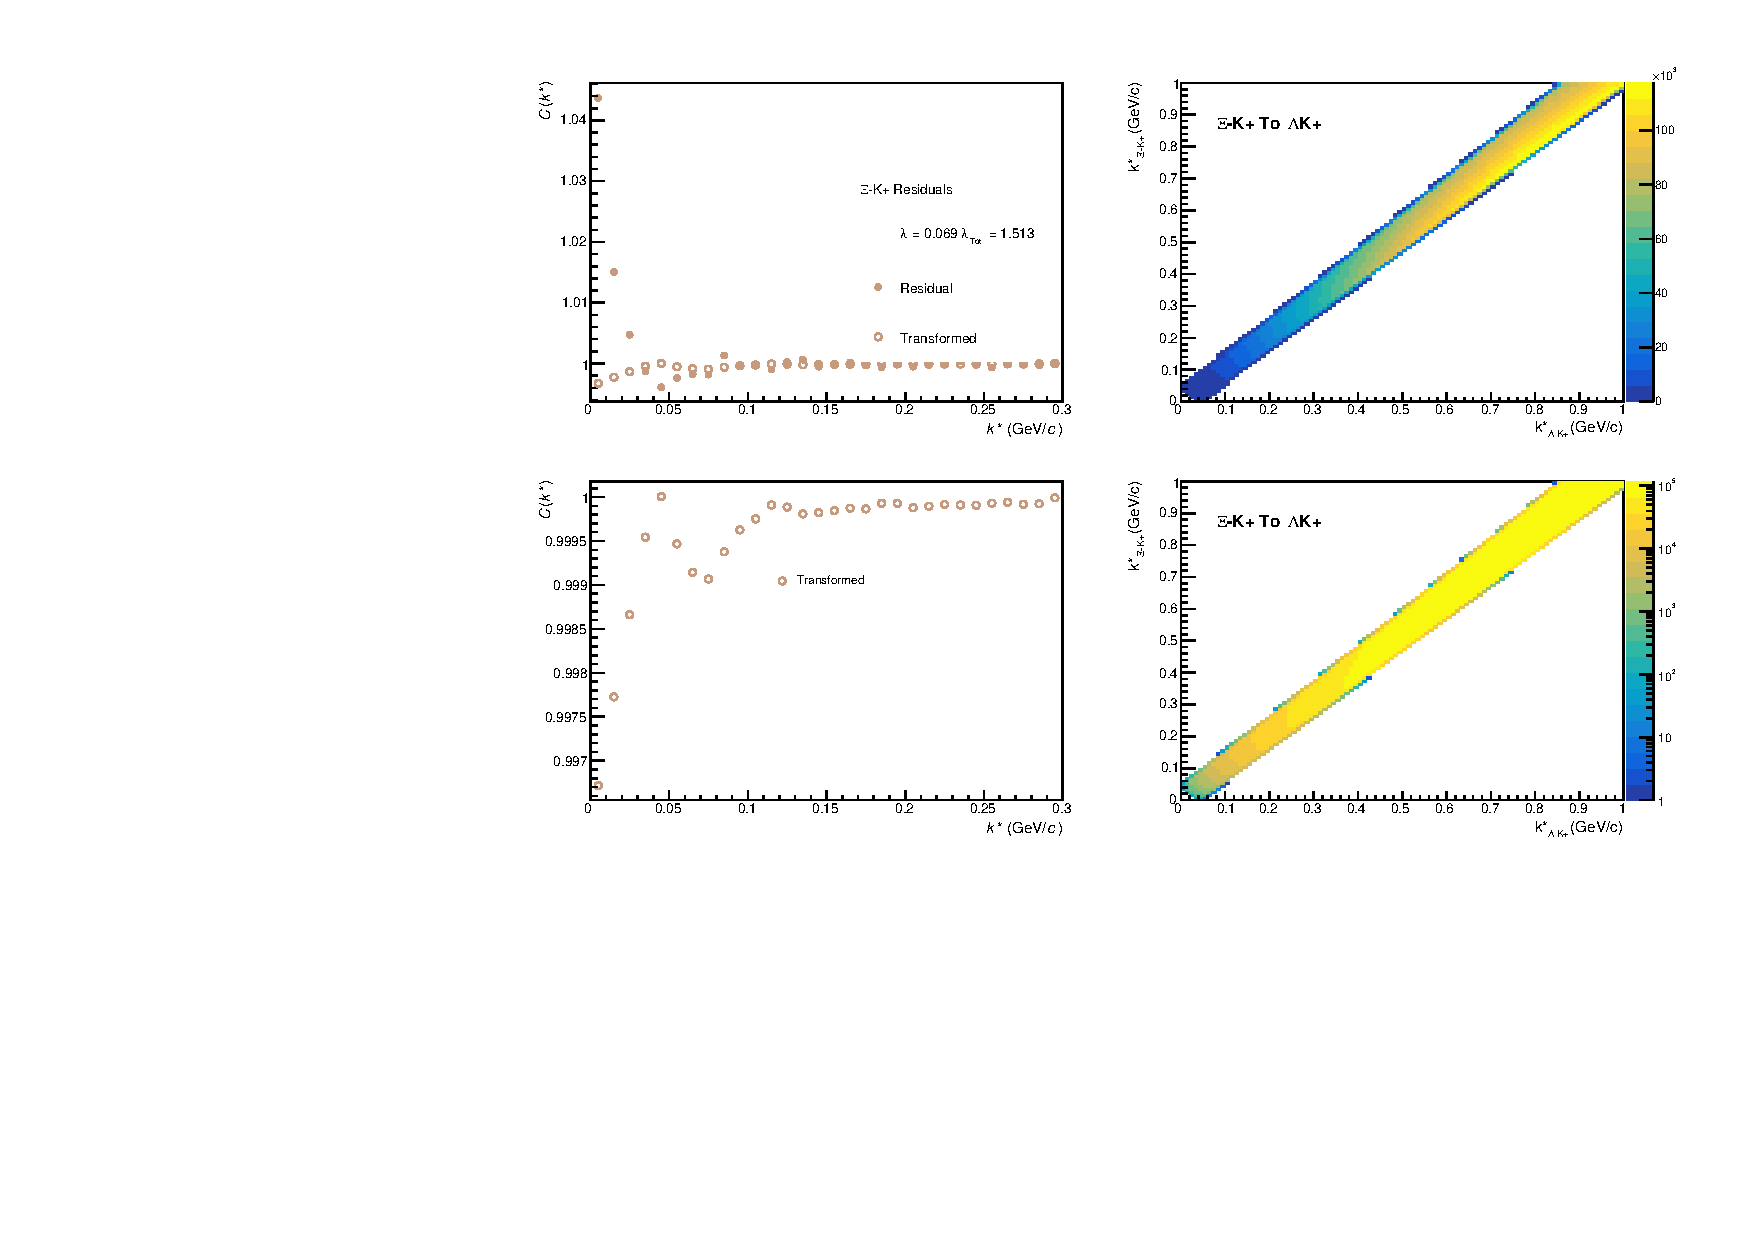
\includegraphics[width=\textwidth]{9_AdditionalFigures/Figures/Residuals/LamKchP/Residuals_LamKchP_0010_XiKchP_MomResCrctn_NonFlatBgdCrctn_10Res_PrimMaxDecay4fm_UsingXiDataAndCoulombOnly.pdf}
  \caption[Residuals: $\Xi^{-}$K$^{+}$ to $\Lambda$K$^{+}$ (0-10\% Centrality)]{Residuals: $\Xi^{-}$K$^{+}$ to $\Lambda$K$^{+}$ (0-10\% Centrality)}
  \label{fig:Res_LamKchP_0010_XiCKchP}
\end{figure}


\begin{figure}[h]
  \centering
  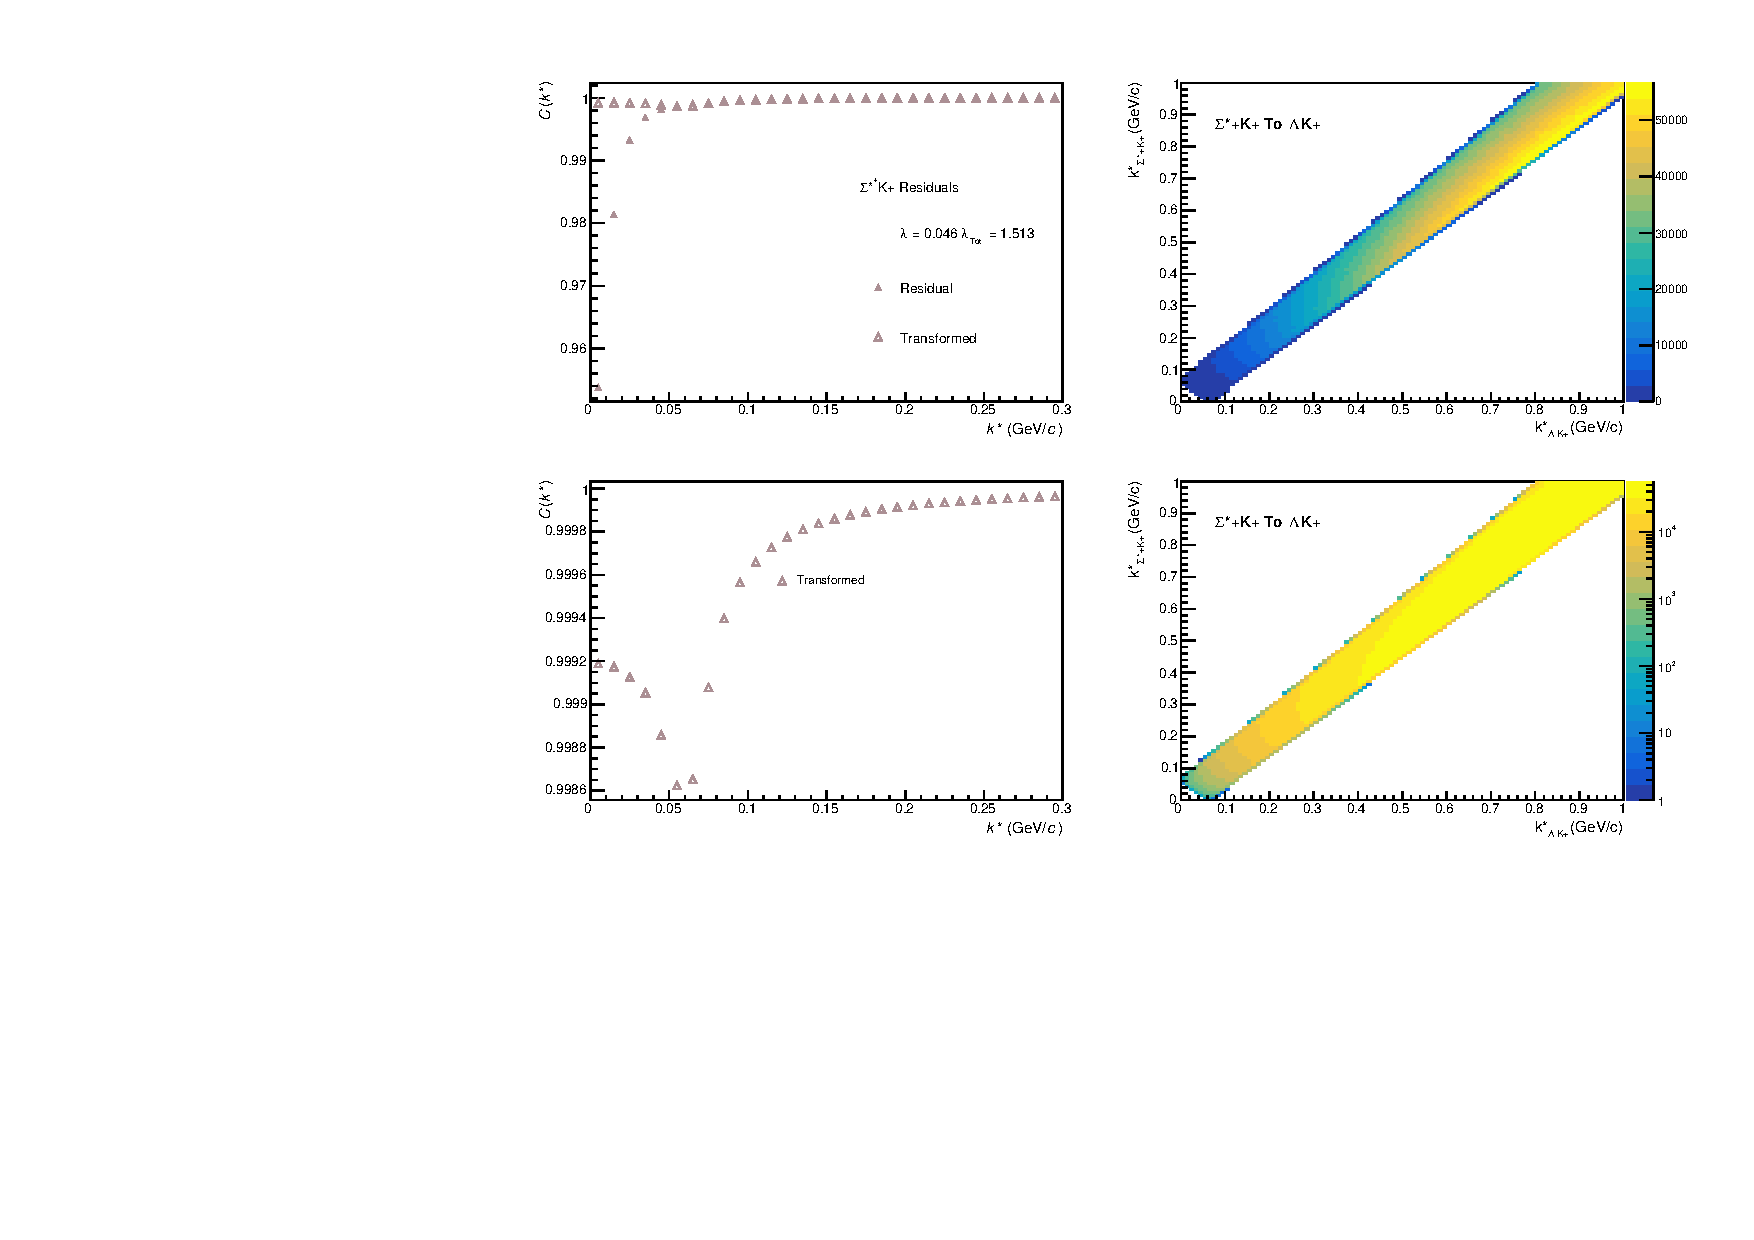
\includegraphics[width=\textwidth]{9_AdditionalFigures/Figures/Residuals/LamKchP/Residuals_LamKchP_0010_SigStPKchP_MomResCrctn_NonFlatBgdCrctn_10Res_PrimMaxDecay4fm_UsingXiDataAndCoulombOnly.pdf}
  \caption[Residuals: $\Sigma^{*+}$K$^{+}$ to $\Lambda$K$^{+}$ (0-10\% Centrality)]{Residuals: $\Sigma^{*+}$K$^{+}$ to $\Lambda$K$^{+}$ (0-10\% Centrality)}
  \label{fig:Res_LamKchP_0010_SigStPKchP}
\end{figure}

\begin{figure}[h]
  \centering
  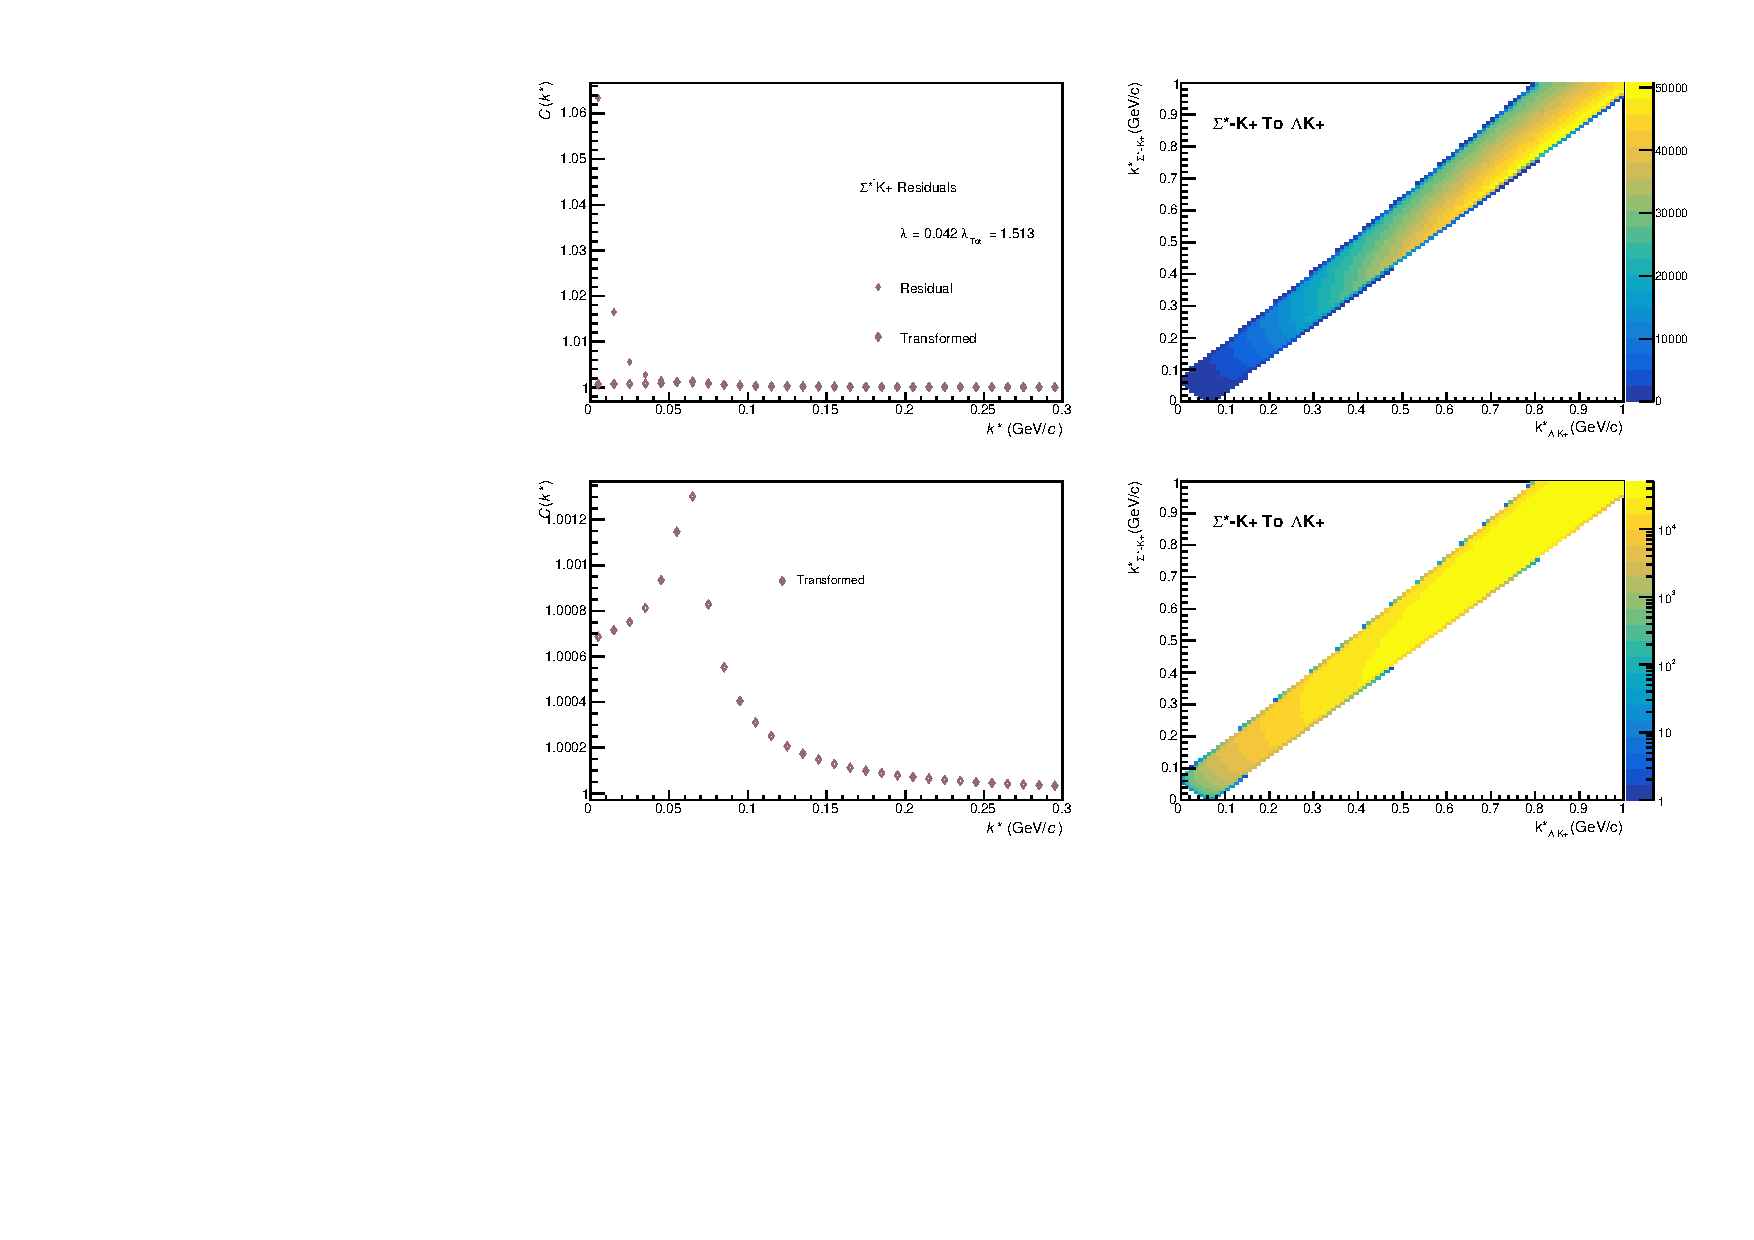
\includegraphics[width=\textwidth]{9_AdditionalFigures/Figures/Residuals/LamKchP/Residuals_LamKchP_0010_SigStMKchP_MomResCrctn_NonFlatBgdCrctn_10Res_PrimMaxDecay4fm_UsingXiDataAndCoulombOnly.pdf}
  \caption[Residuals: $\Sigma^{*-}$K$^{+}$ to $\Lambda$K$^{+}$ (0-10\% Centrality)]{Residuals: $\Sigma^{*-}$K$^{+}$ to $\Lambda$K$^{+}$ (0-10\% Centrality)}
  \label{fig:Res_LamKchP_0010_SigStMKchP}
\end{figure}

\begin{figure}[h]
  \centering
  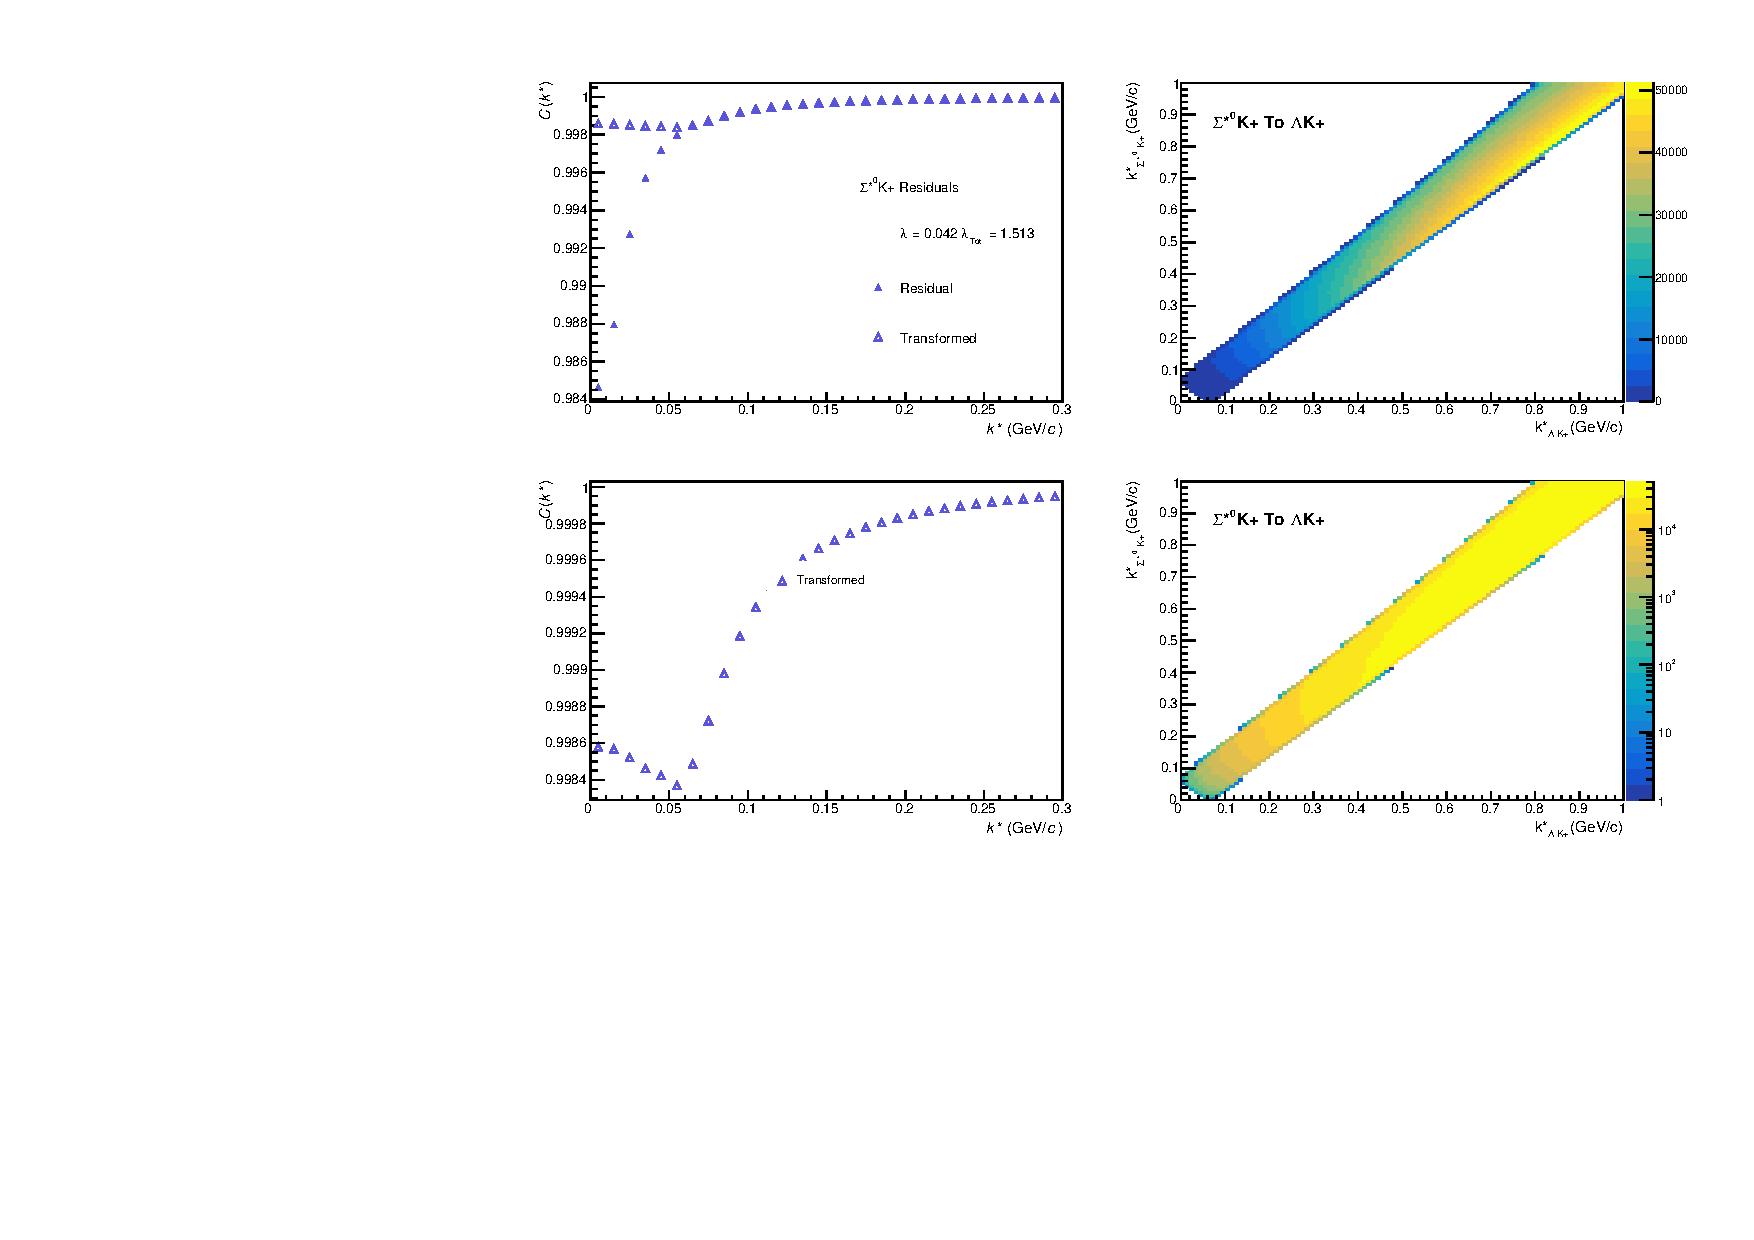
\includegraphics[width=\textwidth]{9_AdditionalFigures/Figures/Residuals/LamKchP/Residuals_LamKchP_0010_SigSt0KchP_MomResCrctn_NonFlatBgdCrctn_10Res_PrimMaxDecay4fm_UsingXiDataAndCoulombOnly.pdf}
  \caption[Residuals: $\Sigma^{*0}$K$^{+}$ to $\Lambda$K$^{+}$ (0-10\% Centrality)]{Residuals: $\Sigma^{*0}$K$^{+}$ to $\Lambda$K$^{+}$ (0-10\% Centrality)}
  \label{fig:Res_LamKchP_0010_SigSt0KchP}
\end{figure}


\begin{figure}[h]
  \centering
  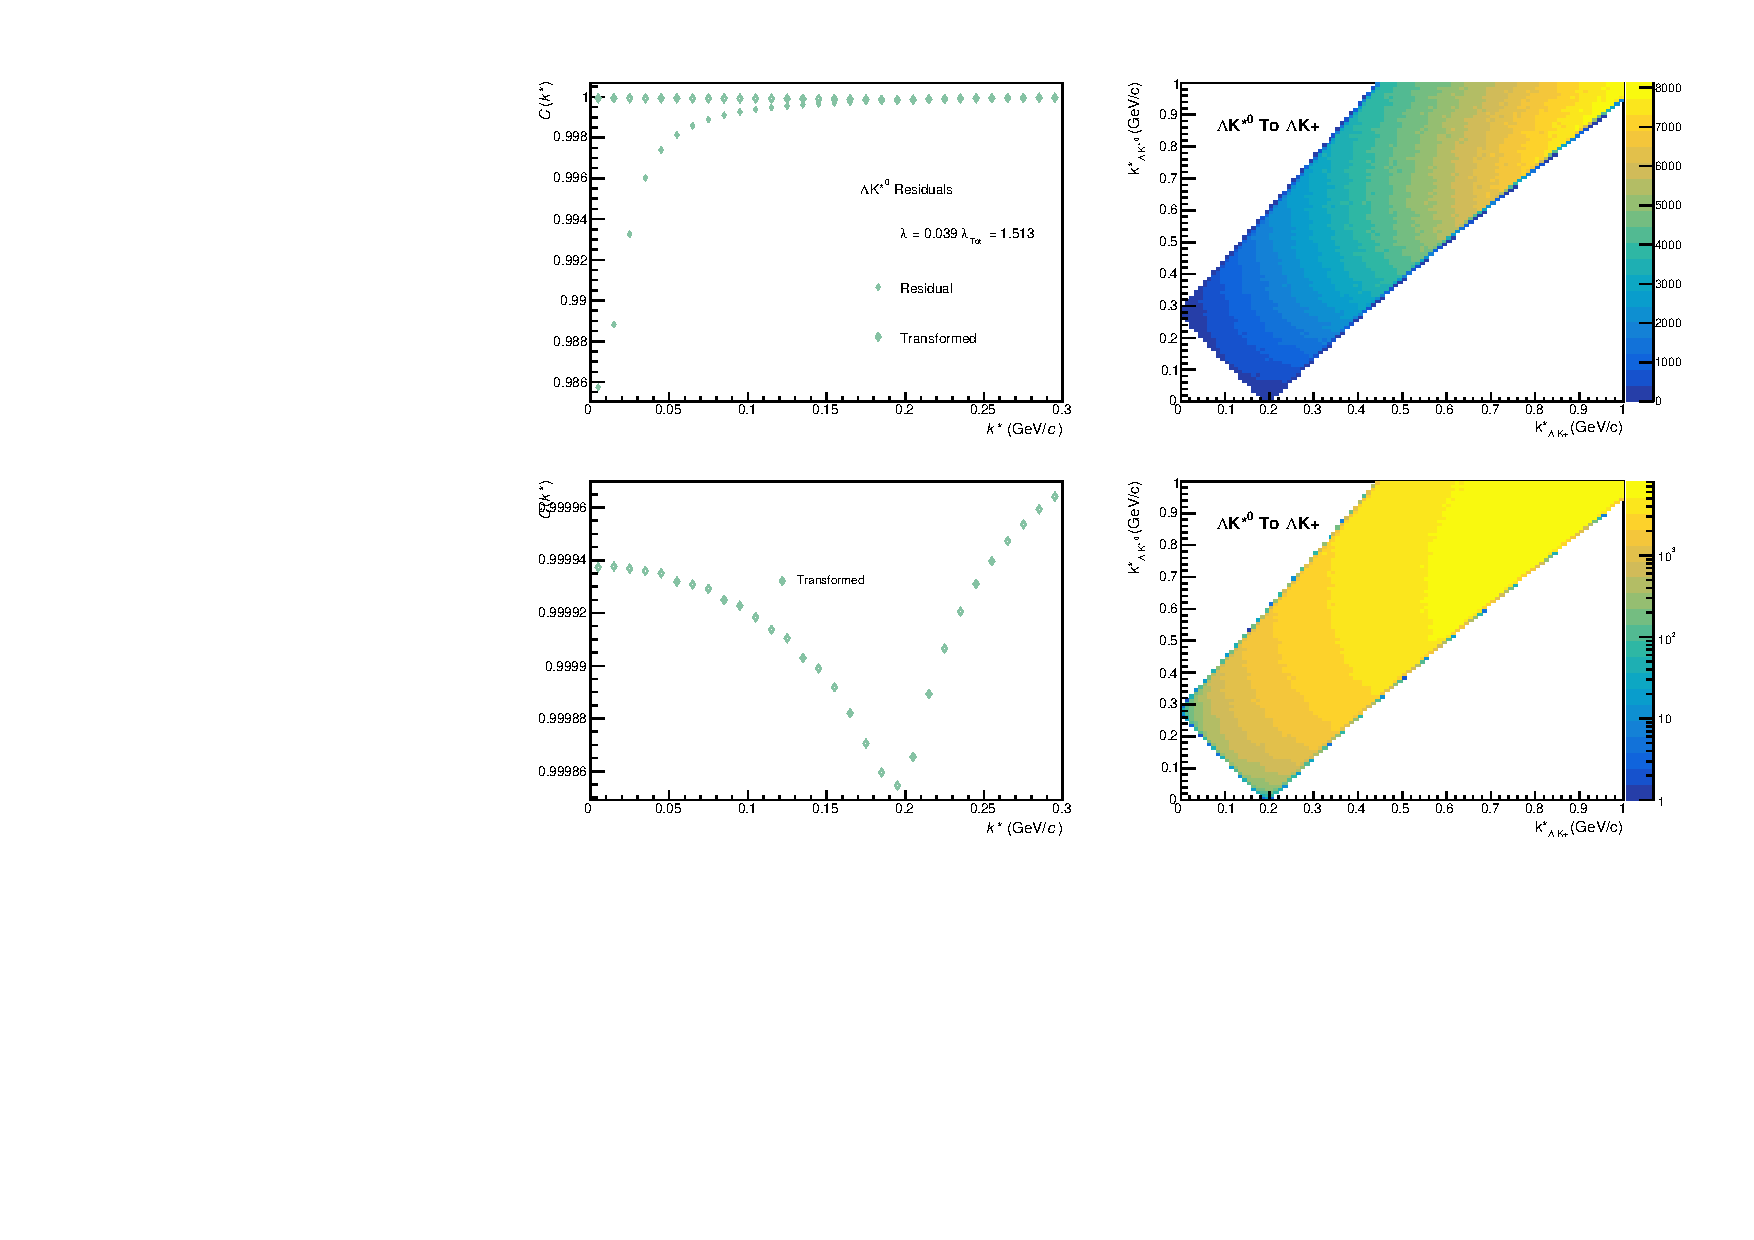
\includegraphics[width=\textwidth]{9_AdditionalFigures/Figures/Residuals/LamKchP/Residuals_LamKchP_0010_LamKSt0_MomResCrctn_NonFlatBgdCrctn_10Res_PrimMaxDecay4fm_UsingXiDataAndCoulombOnly.pdf}
  \caption[Residuals: $\Lambda$K$^{*0}$ to $\Lambda$K$^{+}$ (0-10\% Centrality)]{Residuals: $\Lambda$K$^{*0}$ to $\Lambda$K$^{+}$ (0-10\% Centrality)}
  \label{fig:Res_LamKchP_0010_LamKSt0}
\end{figure}


\begin{figure}[h]
  \centering
  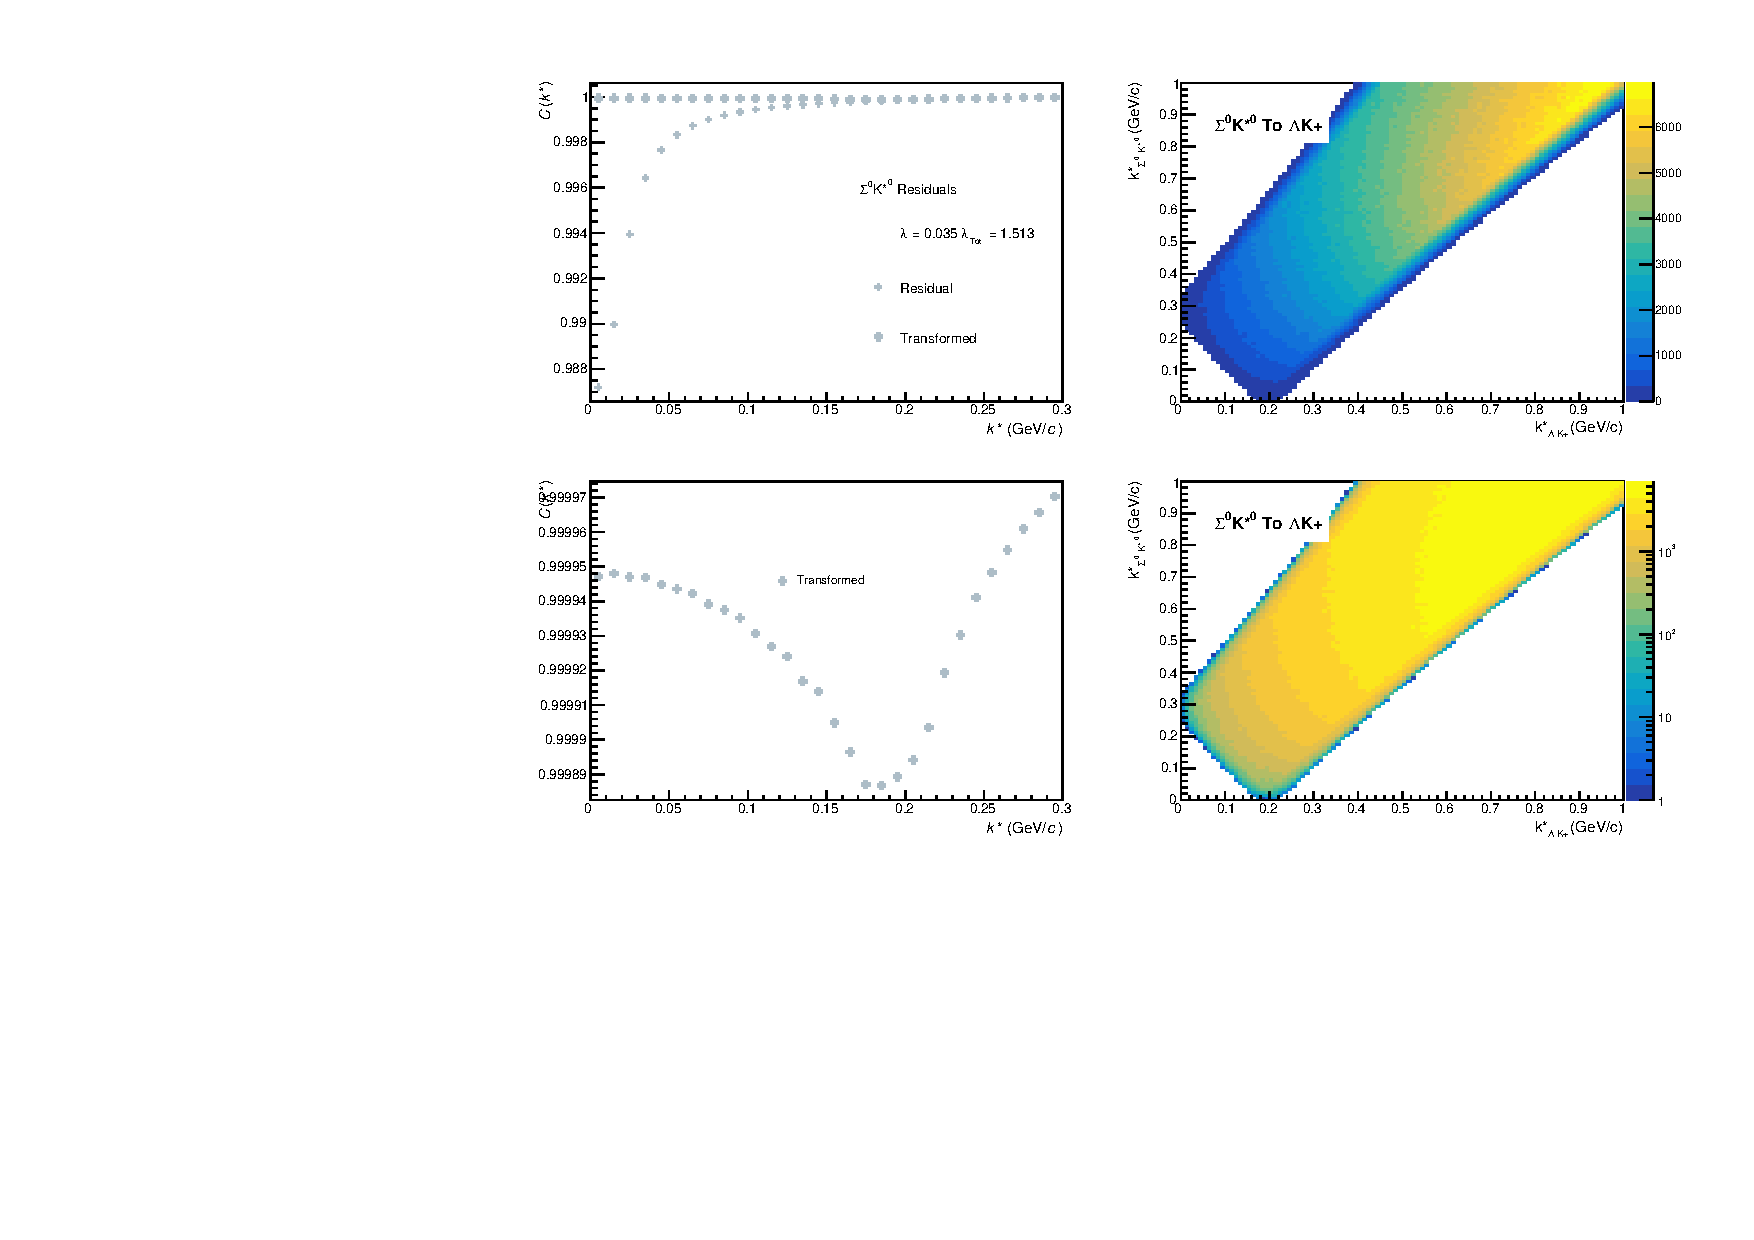
\includegraphics[width=\textwidth]{9_AdditionalFigures/Figures/Residuals/LamKchP/Residuals_LamKchP_0010_Sig0KSt0_MomResCrctn_NonFlatBgdCrctn_10Res_PrimMaxDecay4fm_UsingXiDataAndCoulombOnly.pdf}
  \caption[Residuals: $\Sigma^{0}$K$^{*0}$ to $\Lambda$K$^{+}$ (0-10\% Centrality)]{Residuals: $\Sigma^{0}$K$^{*0}$ to $\Lambda$K$^{+}$ (0-10\% Centrality)}
  \label{fig:Res_LamKchP_0010_Sig0KSt0}
\end{figure}


\begin{figure}[h]
  \centering
  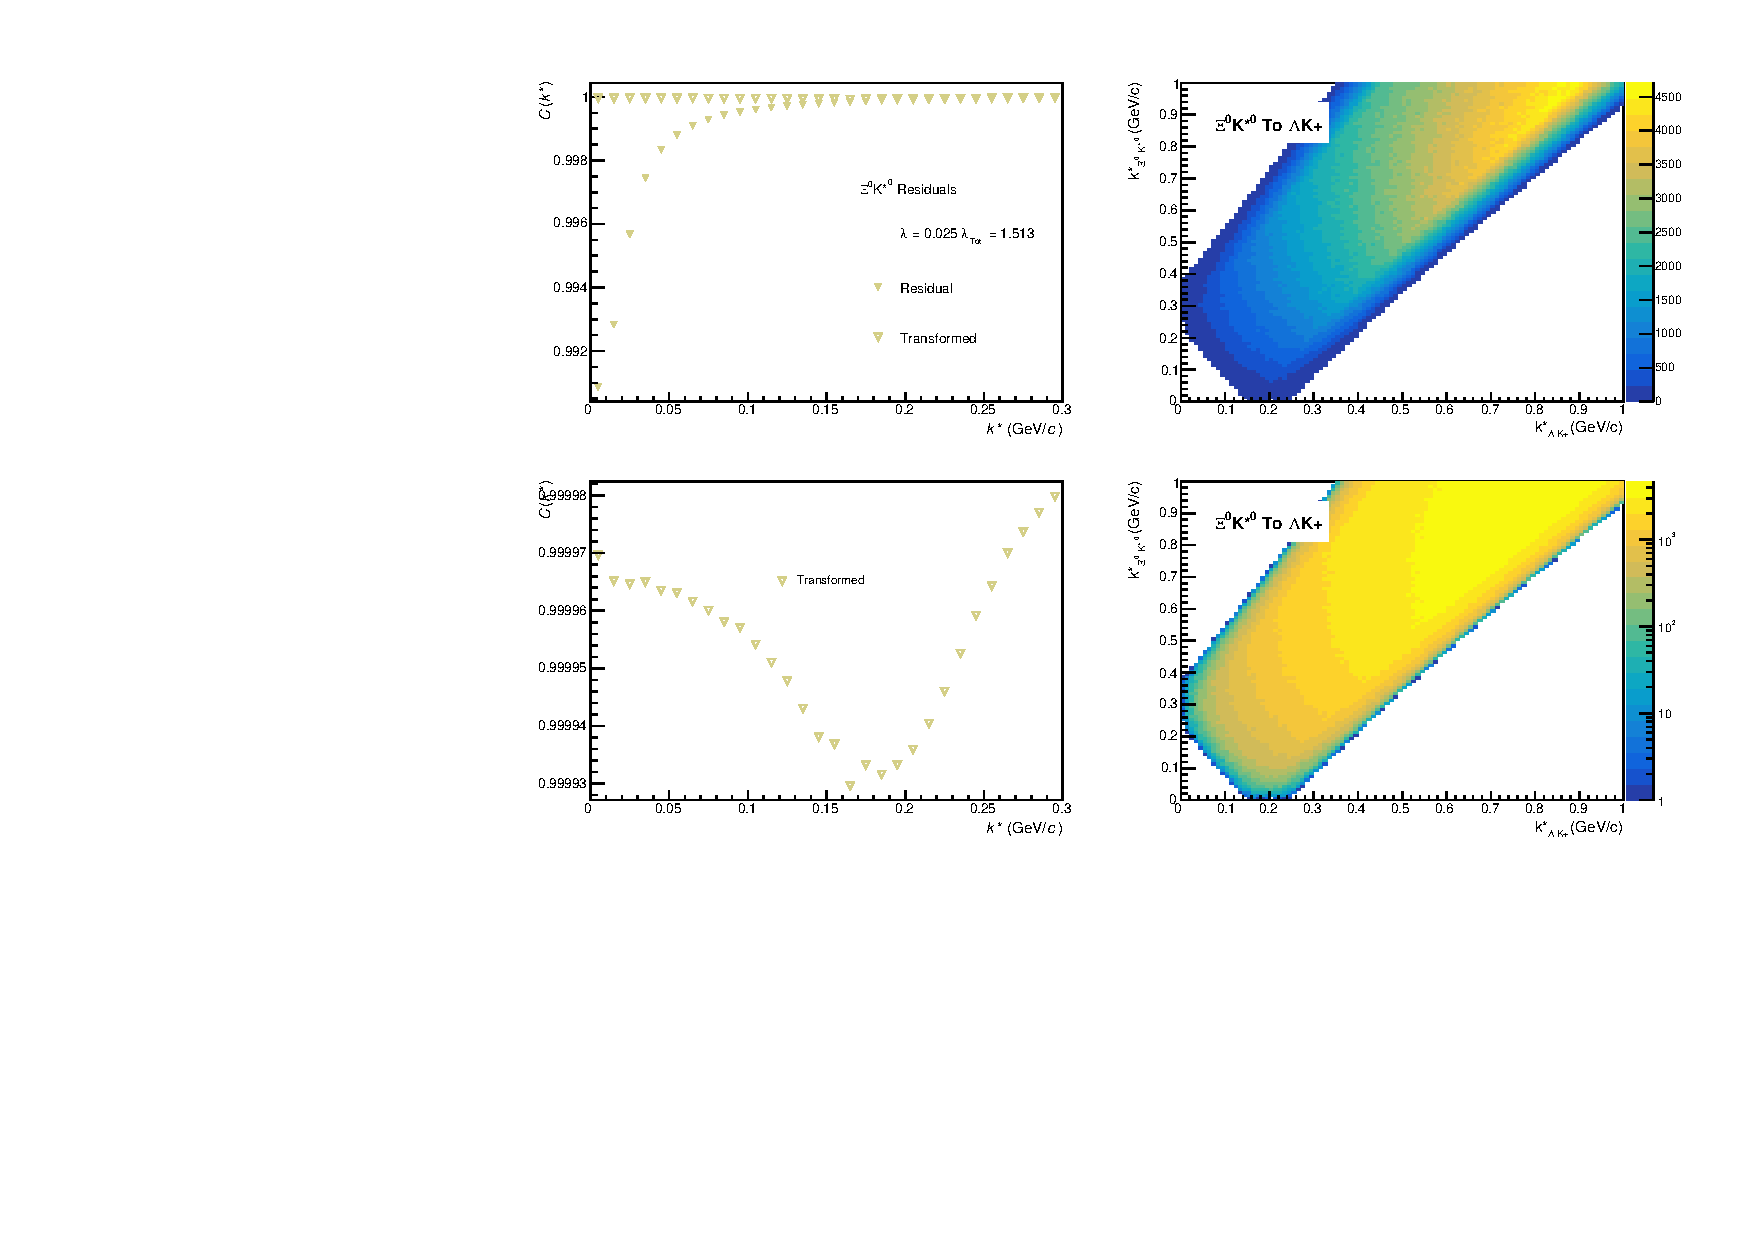
\includegraphics[width=\textwidth]{9_AdditionalFigures/Figures/Residuals/LamKchP/Residuals_LamKchP_0010_Xi0KSt0_MomResCrctn_NonFlatBgdCrctn_10Res_PrimMaxDecay4fm_UsingXiDataAndCoulombOnly.pdf}
  \caption[Residuals: $\Xi^{0}$K$^{*0}$ to $\Lambda$K$^{+}$ (0-10\% Centrality)]{Residuals: $\Xi^{0}$K$^{*0}$ to $\Lambda$K$^{+}$ (0-10\% Centrality)}
  \label{fig:Res_LamKchP_0010_Xi0KSt0}
\end{figure}

\begin{figure}[h]
  \centering
  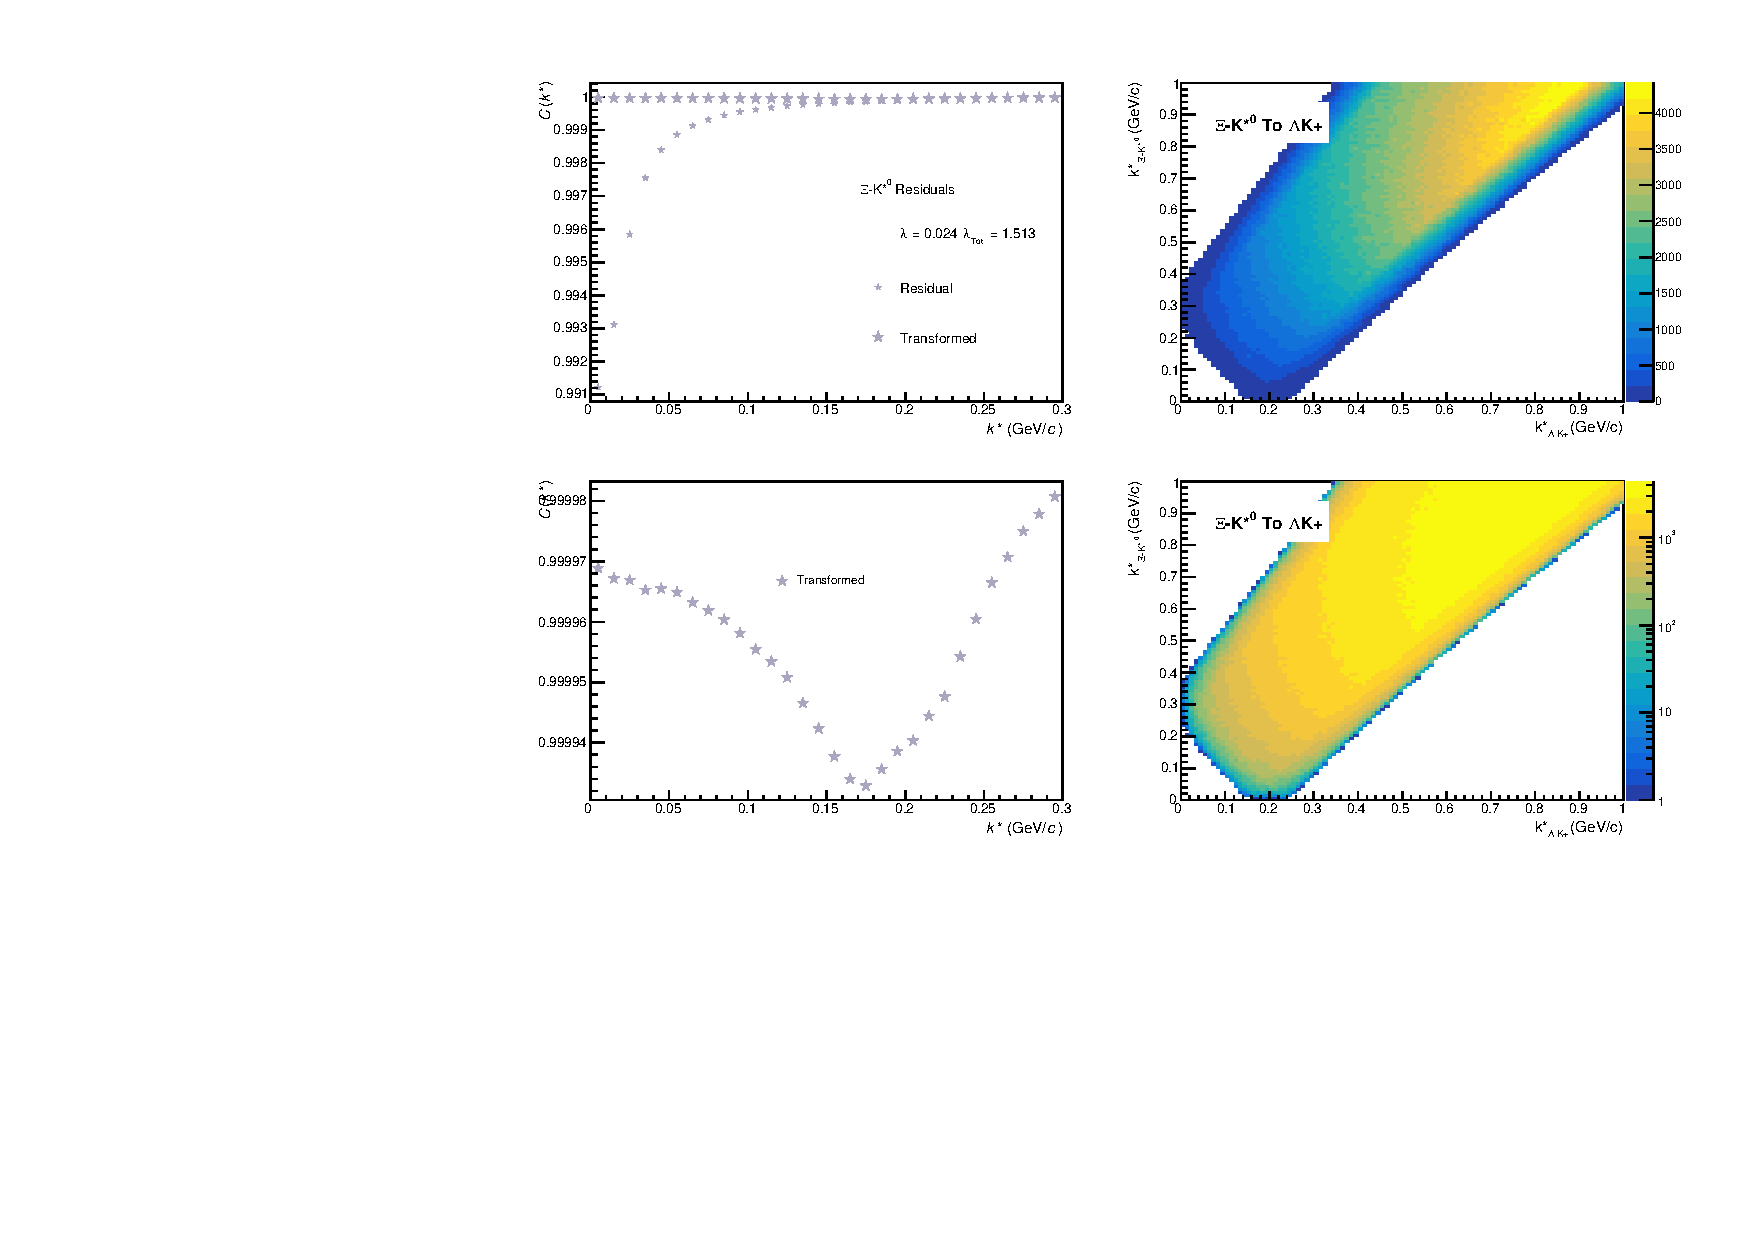
\includegraphics[width=\textwidth]{9_AdditionalFigures/Figures/Residuals/LamKchP/Residuals_LamKchP_0010_XiKSt0_MomResCrctn_NonFlatBgdCrctn_10Res_PrimMaxDecay4fm_UsingXiDataAndCoulombOnly.pdf}
  \caption[Residuals: $\Xi^{-}$K$^{*0}$ to $\Lambda$K$^{+}$ (0-10\% Centrality)]{Residuals: $\Xi^{-}$K$^{*0}$ to $\Lambda$K$^{+}$ (0-10\% Centrality)}
  \label{fig:Res_LamKchP_0010_XiCKSt0}
\end{figure}


\end{document}